%! Author = danjane
%! Date = 17.09.22

\documentclass[10pt]{article}

\usepackage{amsmath, amsfonts}
\usepackage{cmbright}

\usepackage{tcolorbox}


\usepackage{tikz}
\usetikzlibrary{positioning}
\tikzset{
  desk/.style={
    shape=rectangle,
    draw,
    font=\footnotesize,
    minimum width=2cm,
    minimum height=1cm,
  },
  block/.style={
  draw, rectangle, minimum height=1cm
  }
}
\usepackage{adjustbox}

\usepackage{pdflscape}


\begin{document}

\tableofcontents



\section{Introduction}

From the classic teaching literature, Bucheton and Soulé have described the act of teaching as a multi-agenda game of postures requiring good preparation and excellent micro-decisions \cite{BS09}. In their model, they identify the crucial roles of the teacher in controlling the cadence, the atmosphere, the scaffolding and the relationships during the class, and how each supports the learning objective. Many of the teacher's most time-consuming tasks do not take place in the classroom: good preparation and strong follow-ups (auto-reflection, marking, parent-teacher interactions) work to support and complement the overall success of the student learning process.

For example, teacher responsibilities include the ability to [TODO: citation needed]
\begin{itemize}
\item plan and implement effective classroom management practices,
\item design and implement effective strategies to develop independent learners,
\item engage students in active, hands-on, creative problem-based learning,
\item build students’ ability to work collaboratively with others,
\item maintain a safe, orderly environment conducive to learning,
\item adapt instruction/support to students’ differences in development, learning styles, strengths and needs, and
\item write student reports to guide changes in instruction and practice, and to improve student learning.
\end{itemize}

Many of these tasks are "ripe for automation" \cite[p.? TODO]{Swei15}, although I would also accept that some of these tasks should \textbf{not} be automated (even if they can be). As John Hattie explains in \emph{Visible Learning} \cite{Hat12}, \emph{``Expert teachers monitor learning and provide feedback.''} In my opinion writing student reports are a perfect example of a necessary evil: although time consuming (and potentially stressful) for the teacher, writing a student report forces the teacher to reflect on the progress of the student and at the same time manage the expectations of all partners - student, teacher, management and parent.

So which tasks should be automated? Why? And for whom? When I first started teaching, my natural character led to two bad teaching practices: I found it difficult to engage with the quieter, more reserved students; and I was so busy answering student questions that I left little time for taking notes. I felt my teaching (and so hopefully also my students' learning experience) would benefit from a tool which tracked my interactions in class in an attempt to shift the focus away from the "louder" students. 

TODO: discussion on equality for students, and \cite{Hat12} on answering too quickly.

But if I start recording a brief comment at an opportune moment after a positive (or negative) interaction with a set of students, I could also use this to build a reminder of the interactions per student: a useful capability when planning lessons, writing reports, and especially for parent evenings.

For the Master's thesis project undertaken for the GymInf formation, I chose to build a suite of tools to support a range of teacher tasks including capturing key interaction information, building individual student reports, suggesting teacher-student interactions for upcoming classes, organising seating plans, and creating spreadsheets of marks. 

\

I will now explain the layout of this thesis. In sections \ref{inout} and \ref{actions} I outline the planned architecture of the system, explaining how it can be built incrementally. While I sometimes take the opportunity to explore alternative solutions, in general I mainly explain and defend my decisions.

\

The tools will be coded in Python. This choice of language is mainly because Python is the language we teach our students, see section \ref{language}, and I would like to take this opportunity to consolidate my Python skillset.

\

I also wanted to use this thesis to improve my coding style, exploring the industry technique of \emph{test driven development} as explained in section \ref{tdd}. The majority of my contemporaries from university who ended up in university have highly recommended this coding style, and while it has disadvantages (as discussed later) there are strong reasons to having it as an option \cite{Amman16}. TODO proper link to book.

\

TODO intro for chaps 7 and 8

\

Given the limited resources of this masters' thesis, not all of the desired functionality has been delivered. These missing features are described in section \ref{notdone}. Please note that the current codebase was designed with these features in mind, and that existing code should require minimal changes to incorporate these features as they are added.

\section{Project scope}

As Robinson points out in \emph{BOSCARD: a scoping tool} \cite{Rob19}, for a project to be effective and efficient it is necessary (but alas not sufficient) to be clear about the project's aims from the start. BOSCARD is an acronym for background, objectives, scope, constraints, assumptions, risks, and deliverables. Although an industry standard, Robinson claims that the origins of this approach to project planning are unclear but likely originated with the consulting company Cap Gemini in the 1980s \cite[p. 181]{Rob19}.

\subsection{Background}
\emph{Provide background information that includes the reasons for creating the project and mentions the key stakeholders who will benefit from the project result.}

I am doing master's thesis in Computing and have chosen to create a suite of tools to aid teachers. These will be implemented through the \emph{teacher assisting tools} system, called TAT. This will be aimed at assisting  myself and other teachers in their daily work.

\subsection{Objectives} 
\emph{Describe the project goals and link each of them with related, SMART project objectives.}

There are common mistakes made by many new teachers, for example 
\begin{itemize}
\item answering student questions immediately rather than leaving time for the class to think,
\item allowing a subset of students to monopolise class interactions, and
\item taking inadequate notes during class.
\end{itemize}
I will build the TAT system to help teachers to overcome these issues. As well as recording student interaction information, the system will also build individual student reports, suggest future teacher-student interactions for upcoming classes, suggest seating plans, and create spreadsheets of marks.

\subsection{Scope} 
\emph{Provide a high-level description of the features and functions that characterize the product, service, or result the project is meant to deliver.}

TAT will be able to:
\begin{itemize}
\item Actions during teaching.
\begin{itemize}
  \item Record, during class, an interaction with a set of students.
  \item Suggest students for focus, see section \ref{output_focus}.
  \item Manually modify the seating plan as required.
 \end{itemize}
 \item Actions outside of teaching.
 \begin{itemize}
  \item Prepare student reports.
  \item Suggest a seating plan. \textbf{Descoped.}
  \item Review previous seating plans.  \textbf{Descoped.}
  \item Prepare an empty spreadsheet for marking and noting an exam.
  \item Collate marks and calculate semester note.
\end{itemize}
\item Actions to set up the class.
\begin{itemize}
  \item Add a class to the list of classes taught.
  \item Configure the class lists.
  \item Suggest a seating plan.  \textbf{Descoped.}
\end{itemize}
\end{itemize}

The TAT backend will be linked to a GUI, run from a single executable file, with a local instance per teacher.

\

TAT will not connect to the internet. TAT will not cover data privacy concerns beyond what is currently used in standard teaching practices in Geneva, see section TODO \ref{data_privacy}.

\

All development and testing will be done on my personal machine, a MacBook Air, and be delivered to the examiner on this platform as he has the same operating system. Any work required to migrate to the school system will not be in the scope of this thesis.

\subsection{Constraints} 
\emph{Identify the specific constraints or restrictions that limit or place conditions on the project, especially those associated with project scope.}

The thesis must be defended and marked by September 8$^{th}$, 2023. Therefore the TAT system must be delivered to my thesis advisor before August 14$^{th}$ 2023. I am writing this thesis and the code for the TAT system alone: while a basic functionality is essential for all objectives, I anticipate future enhancements and even functional additions will occur.

The TAT system will eventually run on the school computers. TODO: find out what they are running. However, for this project all testing will be done on my local machine.

\subsection{Assumptions} 
\emph{Specify all factors that are, for planning purposes, considered to be true. During the planning process, these assumptions will be validated.}

I will assume that classes have at most 24 students, and that the seating plan is arranged in the standard three-by-four blocks of pairs.

\subsection{Risks} 
\emph{Outline the risks identified at the start of the project. Include a quick assessment of the significance of each risk and how to deal with them.}

Given the constraints, and especially the time limit, there is a large risk of some features being dropped from the first version. I want to first deliver basic functionality with a graphical user interface, and then add as many features as possible in the timeframe.

\subsection{Deliverables} 
\emph{Define the key deliverables the project is required to produce to achieve the stated objectives.}

The TAT system will provide a basic GUI over a backend handling the tasks covered in the scope. In particular, the system should at least allow notes to be taken against student names and then suggest pertinent students for focus.

\section{System plan} \label{inout}

In his 2017 book "Clean Architecture" Robert Martin\footnote{Robert Martin likes to be called "Uncle Bob".} is clear about why we invest time in the planning phase of an IT system:
\begin{center}
\emph{"The goal of software architecture is to minimize the human resources required to build and maintain the required system."} \cite[p. 5]{Mart17}
\end{center}


We can analyse a system by connecting its (physical or virtual) inputs and outputs. In this project, we have

\

\begin{minipage}[t]{0.38\textwidth}

\textbf{Inputs}

\begin{itemize}
\item Class lists
\item Commentary on students
\item Seating plan used in class
\item Exam notes and weights
\end{itemize}


\end{minipage}
\hfill
\vline
\hfill
\begin{minipage}[t]{0.48\textwidth}

\textbf{Outputs}

\begin{itemize}
\item Suggested students for focus
\item Suggested seating plans
\item Average notes for the semester
\item Individual student reports
\end{itemize}

\end{minipage}

\vspace{5mm}

The inputs clearly contain sensitive information, and the relevant laws and best practices with regards to student data will be discussed further in Section \ref{dataprivacy}. It is also worth pointing out that the processed data (data during calculations and the outputs) is also sensitive. In general we should try to store as little personal data as possible. TODO citation needed.

\subsection{Explanation of inputs}

\subsubsection{Class lists}
For each class of interest, we need to have a list of students who are members of this class. For each student, it is often useful to store a "given" name with which they like to be called in class. Other information is not essential (gender, age, etc.), and so we will not store it.

\subsubsection{Commentary on students}
During the teaching process, the teacher makes useful judgements about students and groups of students. The teaching process obviously includes contact time during classes, but it can also include thoughts and decisions during the planning process, while marking homework or exams, or while evaluating a lesson \emph{ex-post}.

Comments could take the form
\begin{itemize}
\item Excellent definition of Pythagoras' Theorem
\item Good explanation of photosynthesis on blackboard
\item Very quick with past continuous exercises
\item Chatting
\item DNF \emph{(homework not done)}
\item Seemed unashamed that he did not know the formula for the area of a triangle.
\end{itemize}

To each comment should be associated the student, the class and the date. Thinking ahead, It would be very useful to also include whether or not the comment was positive or negative: see the "focus" and "report" outputs, respectively sections \ref{output_focus} and \ref{output_report}.

\subsubsection{Seating plan used in class}
Especially at the start of the year, but also just after holidays, it can be difficult to remember the given names of students. By asking the students to follow a seating plan \emph{and then having this seating plan to hand,} the teacher has an easy way to refer to students by their given name. At the start of the year this also helps the teacher in learning the names. See figure \ref{seatingplan} on page \pageref{seatingplan} for an example of a seating plan created using the tikz package of LaTeX. As far as possible, I followed the format of seating plans used during exams at Collège Rousseau : thus the seating plan layout should be familiar to both students and teachers.

\begin{figure} \label{seatingplan} \centering
\begin{adjustbox}{width=0.8\textwidth, frame=1pt 10pt}
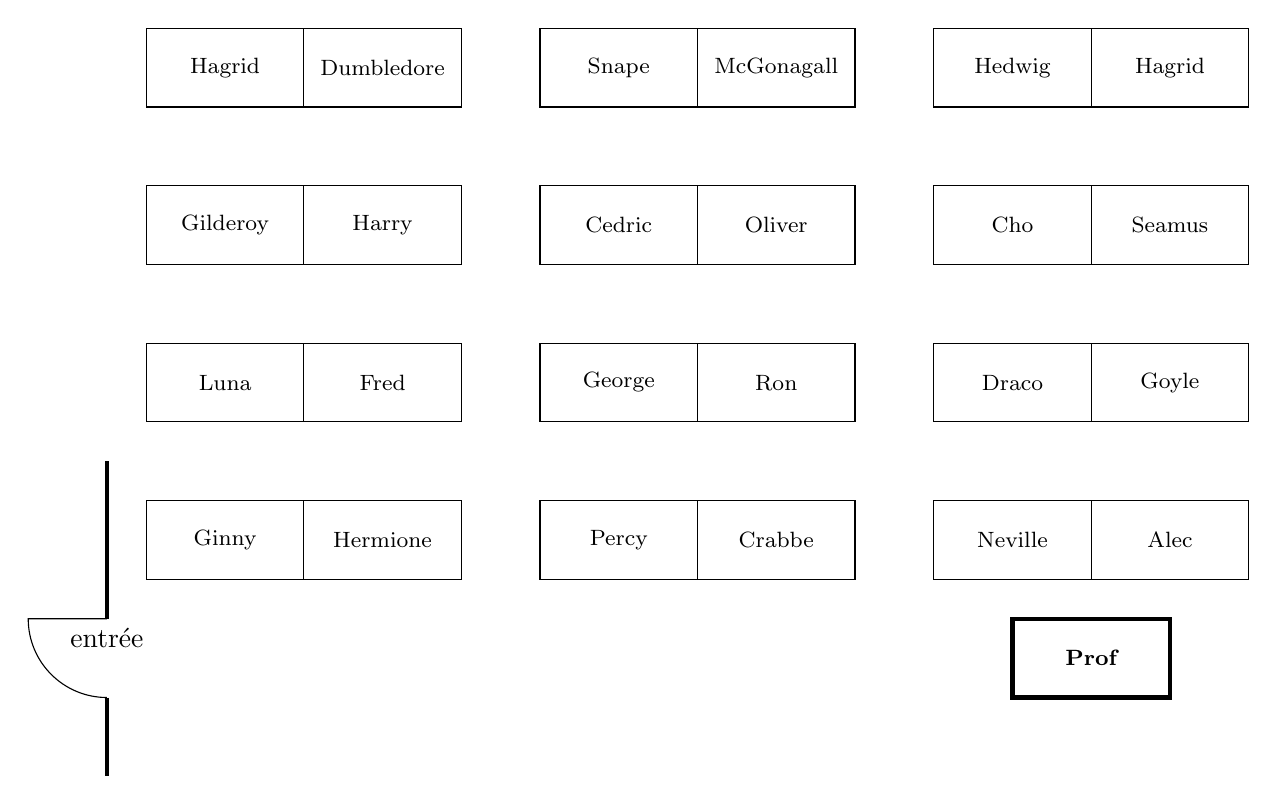
\begin{tikzpicture}

% Students
\node[desk] at (0,0) {Ginny};
\node[desk] at (2,0) {Hermione};
\node[desk] at (5,0) {Percy};
\node[desk] at (7,0) {Crabbe};
\node[desk] at (10,0) {Neville};
\node[desk] at (12,0) {Alec};
\node[desk] at (0,2) {Luna};
\node[desk] at (2,2) {Fred};
\node[desk] at (5,2) {George};
\node[desk] at (7,2) {Ron};
\node[desk] at (10,2) {Draco};
\node[desk] at (12,2) {Goyle};
\node[desk] at (0,4) {Gilderoy};
\node[desk] at (2,4) {Harry};
\node[desk] at (5,4) {Cedric};
\node[desk] at (7,4) {Oliver};
\node[desk] at (10,4) {Cho};
\node[desk] at (12,4) {Seamus};
\node[desk] at (0,6) {Hagrid};
\node[desk] at (2,6) {Dumbledore};
\node[desk] at (5,6) {Snape};
\node[desk] at (7,6) {McGonagall};
\node[desk] at (10,6) {Hedwig};
\node[desk] at (12,6) {Hagrid};


% Prof
\node[desk, ultra thick] at (11, -1.5) {\bfseries Prof};

% Door
\draw[ultra thick] (-1.5,1) -- (-1.5, -1);
\draw[ultra thick] (-1.5,-2) -- (-1.5, -3);
\draw (-1.5,-2) arc (270:180:1) -- (-1.5,-1) node[below] {entrée};

\end{tikzpicture}
\end{adjustbox}

\caption{Example of a seating plan, created with the Tikz package of \LaTeX}

\end{figure}





\subsubsection{Exam notes}

The individual exam results will be needed in order to calculate the average note for each student for each semester, section \ref{output_notes}. We will also need the weighting associated with each exam, and by including the date of the exam we can check the progression of students, section \ref{output_report}.




\subsection{Explanation of outputs}

\subsubsection{Suggested students for focus} \label{output_focus}

As a student teacher, I found it hard to balance my time equitably among the students in a class. Certain students, perhaps those who were louder or more confident, tended to capture my attention. By keeping a record of my interactions with students, it was possible to estimate an ordering of students by recent interactions, and so indicate students who require teacher \emph{focus} during the next set of teacher-student interactions (probably during the next class).

This \emph{focus} can be very simple: these are the students to whom the teacher addresses the opening questions. These opening questions can revise topics from the last lesson or prepare the students for the ideas to be tackled in this lesson. Students who respond positively to an early question are much more likely to volunteer answers later in the class TODO citation needed.

\

Let us model the interactions with a given student by simply counting the number of interactions on a given day.

\begin{tcolorbox}
Comments:

01/06/2023 Harry gives conclusion of Pythag \\
01/06/2023 Harry, Ron correct calc litt \\
04/06/2023 Ron calculates angles in triangle \\
08/06/2023 Harry calculates hypotenuse
\end{tcolorbox}
We define a function $f_H : \mbox{Dates} \to \mathbb{N}$ to count the interactions with Harry
$$ f_{H}(d) = \left\{ \begin{matrix} 2 &  \mbox{if} & d=\mbox{01/06/2023} \\ 1 & \mbox{if} & d=\mbox{08/06/2023}  \\ 0 && \mbox{otherwise.} \end{matrix} \right. $$
and a corresponding function $f_R$ for the interactions with Ron
$$ f_{R}(d) = \left\{ \begin{matrix} 1 &  \mbox{if} & d=\mbox{01/06/2023}  \\ 1 &  \mbox{if} & d=\mbox{04/06/2023}  \\  0 && \mbox{otherwise.} \end{matrix} \right. $$

On a given date $t$ we would like to create a weight operator, $W_t$, which would map these functions to a real number. This operator should measure the number of recent interactions, giving more weight if there have been more interactions. For example, Harry has had more interactions than Ron and so we expect $W_t(f_H) > W_t(f_R)$.

Consider calculating the students for focus just before the holidays or just after the holidays. Assuming the list of comments has not changed, then ideally the \textbf{ordering} of the students by weight would not change. Thus the students for focus should not be dependant on when the algorithm was run. A straightforward property with this behaviour is that all weights change by the same constant. In probability, this is called the \emph{memoryless} property \cite{Norr98} and implies an exponential weighting of the counts:
$$ W_t(f) = \sum_{d \in \mathcal{D}} f(d) \, e^{k(d-t)} $$
where we sum over all dates\footnote{Clearly, as the number of comments is finite this is really a finite sum.}  and $k>0$ is a constant. Then recalculating the weights after $n$ days gives
$$W_{t+n}(f) = \sum_{d \in \mathcal{D}} f(d) \, e^{k(d-(t+n))} =  e^{-kn} \cdot \sum_{d \in \mathcal{D}} f(d) \, e^{k(d-t)} = e^{-kn} \cdot  W_t(f),$$
so all weights are rescaled by $e^{-kn}$ which does not depend on $f$.

To pick the constant $k$, consider the desired relative weighting between a student to whom we made a comment yesterday, and another who received two comments quite a while ago (but two comments on the same day). How much time should pass in order that both students receive the same weight? Completely subjectively, I assume one week should pass, which gives
$$1 e^{0k} = 2 e^{-7k} \Rightarrow k = \frac{1}{7} \ln {2}  \approx 0.1.$$ 

Ideally negative interactions should \textbf{not} be counted in this weighting; otherwise "difficult" students would be unlikely to ever be chosen for positive interactions.

\subsubsection{Suggested seating plans}

Most classes have 24 students arranged in 12 pairs, with the 12 pairs at desks arranged in 3 columns by 4 rows, see figure \ref{seatingplan} on page \pageref{seatingplan}. There are two obvious seating arrangements : using the ordering from the class list\footnote{The class list is alphabetic on surname. However, due to data privacy concerns the system does not have access to the surname: it only has the email username, see section \ref{dataprivacy}. The alphabetic ordering of the usernames is not necessarily the same as the alphabetic ordering of the fullnames. To avoid this problem I use the class list ordering directly rather than the usernames.} or using a random seating plan. For testing and repeatability it is much easier to use a deterministic algorithm, and so I have preferred using the class list as a default seating plan.

As the year progresses we have more information about the students: pairs that work well together, students who work at similar speeds, students which have different strengths. Could we use the student comments and the exam results to suggest seating plans suited to particular lessons?

\subsubsection{Average notes for the semester} \label{output_notes}

The notes in Genevan institutions range between 1.5 and 6.0. The average note for the semester is a weighted sum of the individual notes of the marked exams of the semester. The individual notes are rounded to the nearest half, whereas the \emph{semestriel} notes are rounded to the nearest tenth. Mathematically, 
$$ n_s = R_{0.1} \Bigg(\frac{\sum_{i \in \mathcal{I}_s} \, w_i \cdot n_i }{\sum_{i \in \mathcal{I}_s} \, w_i}\Bigg)$$
where the index runs over the marked exams of the semester, and $R_s$ is the function that rounds to the nearest multiple of $s$.

It is worth pointing out that the rounding function is \emph{not} continuous. While this is obvious, it can make the semestriel note surprisingly sensitive to small changes in individual exam notes. This also true for the end of year note, which is the \textbf{rounded} average of the semestriel notes:
$$n_y = R_{0.1} \Bigg( \frac{n_{s_1} + n_{s_2}}{2} \Bigg).$$
In general the pass mark is 4.0, and the rounding functions are a big advantage for weak students. Consider a concrete example, where before rounding a student receives $3.85$ for the first semester and $3.95$ for the second. Then the final end of year note is
$$n_y = R_{0.1}  \Bigg( \frac{R_{0.1}(3.85) +R_{0.1}(3.95)}{2} \Bigg) = R_{0.1} \Bigg( \frac{3.9 + 4.0}{2} \Bigg) = R_{0.1}(3.95) = 4.0$$
and the student passes! Fingers crossed this also applies to Master's theses.

\

I would like the system to calculate the semestriel and end of year notes for each student.

\subsubsection{Individual student reports} \label{output_report}

It is often useful to have a quick overview of an individual student's progress. Perhaps beforehand, while planning which students will tackle which activities, or afterwards, when analysing the efficacy of a sequence of lessons. More concretely, such an overview would be very useful when meeting parents, when giving notes, and when asked to comment on their progress in the \emph{conseils de classes} at the end of each semester.

Information that would be useful would be the student name, their given name, the class, a list of the comments concerning this student, their exam notes over time, and a graphical visualisation of their progress. Roughly, the overview would include an A4 page per student which looks something like this:

\begin{center}
\begin{tcolorbox}

harry.pttr \hfill \textbf{Harry} \hfill 1ma1df01

\

\small{
01/06/2023 Harry gives conclusion of Pythag \\
01/06/2023 Harry, Ron correct calc litt \\
08/06/2023 Harry calculates hypotenuse
}

\vspace{10mm}

\begin{center}
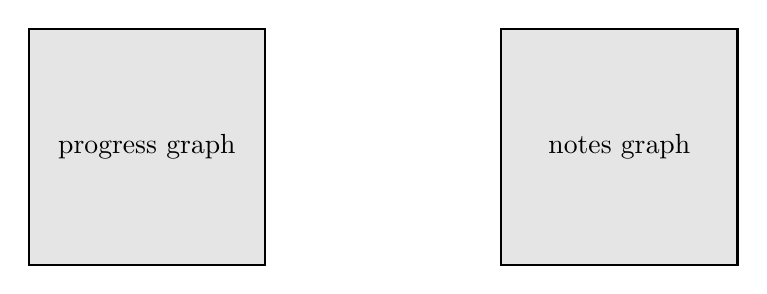
\begin{tikzpicture}

\draw[thick, fill=black!10!white] (0,0) rectangle (3,3) node[pos=0.5] {progress graph};
\draw[thick, fill=black!10!white] (6,0) rectangle (9,3) node[pos=0.5] {notes graph};

\end{tikzpicture}
\end{center}

\end{tcolorbox}
\end{center}


\subsection{Implied structure of backend}

By "backend" I mean the data access layer of the system. By connecting the inputs and outputs we can assess what intermediate processing will be required, and what functionality can be shared. The schematic in figure \ref{dataflowdiagram}, on page \pageref{dataflowdiagram}, is a \emph{Data Flow Diagram} for the TAT system. I have used the Yourdon-Coad notation where the processes (functions) are circles and data is represented by rectangles. Flow of control (transfer of information) is represented by arrows, see \cite{Coad91}.

\begin{figure}[h] \label{dataflowdiagram}
\begin{center}
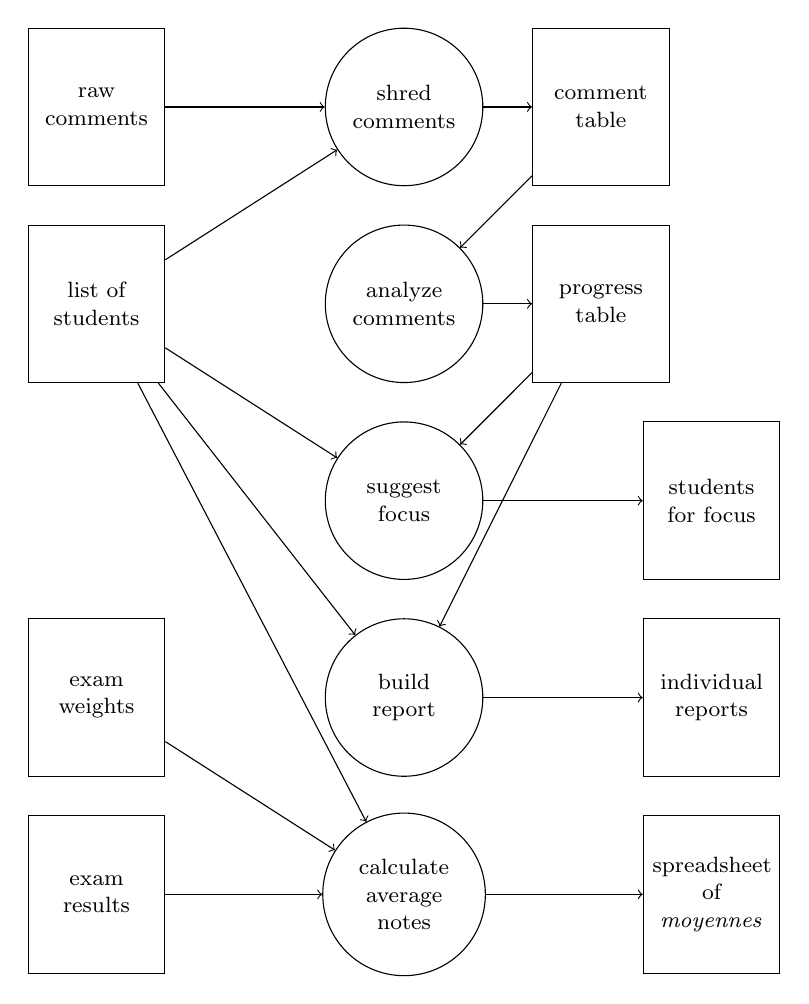
\begin{tikzpicture}[node distance=25mm, every node/.style={draw, text centered, minimum height=20mm, align=center, text width=15mm, font=\fontsize{8}{10}\selectfont}]

\def\datagapmm{40}

\def\function{circle}
\def\datastore{rectangle}
  % Nodes
  \node (comments) [\datastore]{raw comments};
  \node (students) [below of=comments, \datastore] {list of students};
  \node (shred) [right of=comments, xshift=\datagapmm, \function] {shred comments};
  \node (comment_table) [right of=shred, \datastore] {comment table};
  \node (analyze) [below of=shred, \function] {analyze comments};
  \node (progress) [below of=comment_table, \datastore] {progress table};

  % Arrows
  \draw[->] (students) -- (shred);
  \draw[->] (comments) -- (shred);
  \draw[->] (shred) -- (comment_table);
  \draw[->] (comment_table) -- (analyze);
  \draw[->] (analyze) -- (progress);
  
  % Second row
  \node (suggest) [below of=shred, yshift=-25mm, \function] {suggest focus};
  \node (focus) [right of=suggest, xshift=\datagapmm, \datastore] {students for focus};
  \node (build) [below of=suggest, \function] {build report};
  \node (report) [right of=build, xshift=\datagapmm, \datastore] {individual reports};

  \draw[->] (progress) -- (suggest);
  \draw[->] (suggest) -- (focus);
  \draw[->] (progress) -- (build);
  \draw[->] (build) -- (report);
  
  % Third row
  \node (average) [below of=build, \function] {calculate average notes};
  \node (results) [left of=average, xshift=-\datagapmm, \datastore] {exam results};
  \node (weights) [above of=results, \datastore] {exam weights};
  \node (spreadsheet) [right of=average, xshift=\datagapmm, \datastore] {spreadsheet of \emph{moyennes}};
  
  \draw[->] (results) -- (average);
  \draw[->] (weights) -- (average);
  \draw[->] (average) -- (spreadsheet);

  \draw[->] (students) -- (suggest);
  \draw[->] (students) -- (build);
  \draw[->] (students) -- (average);

\end{tikzpicture}

\end{center}
\caption{Data flow diagram for the backend of the TAT system.}
\end{figure}

The data flow diagram in figure \ref{dataflowdiagram}, on page \pageref{dataflowdiagram}, is a very high-level description of a possible system. To make concrete decisions about how to implement the TAT system it will help to define the expected inputs and outputs. In this section I will outline a basic backend based on files.  An implementation based on files is simpler and quicker, and so more suited for a master's project, but in the future I would expect the backend to handle updates via ACID database queries. I will briefly explain the advantages of databases over files in subsection \ref{db}. I will finish this section by touching on the data privacy laws that apply in Geneva; in particular the system will use only a minimum amount of personal data.

\subsubsection{The list of students}
The \textbf{list of students} is a list of students in each class. I will use a text file for each class, storing a list of user-ids for each student. For example, for the class 1in1dfb01 I would create a textfile called "1in1dfb01.txt":
\begin{tcolorbox}[title = 1in1dfb01.txt]
\texttt{harry.pttr\\ronald.wsly\\marie.cr\\richard.fynmn}
\end{tcolorbox}
This also seems a pertinent place to store the given name of each student. Currently the user-id starts with the first name of the student followed by a fullstop followed by (roughly) the consonants of the surname, 
\begin{center}
\texttt{user\_id = firstname + "." + consonants(surname).}
\end{center}
A regular expression of the form \texttt{\textasciicircum
[a-z\textbackslash-]+} strips the student's first name from their user-id. In Python, we use the \texttt{re} package, for example
\begin{center}
\texttt{firstname = re.search(r"\textasciicircum[a-z\textbackslash-]+", user\_id).group(0).capitalize()}
\end{center}
Applying this function to the students above would yield
\begin{center}
\texttt{["Harry", "Ronald", "Marie", "Richard"]}
\end{center}

However, there are two issues with assuming that this function will always yield the given name of a student. Firstly, we do not control how the user-ids are created, and so we cannot guarantee that this function will work in the future. Secondly, a student might want to be called by a different name (for example their second name). 

I decided to add an optional comma-separated second item which designates the given name of a student in a class: this will be the name shown on the seating plan. For example, if Ronald Weasley wished to be called "Ron" and Richard Feynman preferred "Dick", then the file for the class list would be 
\begin{tcolorbox}[title = 1in1dfb01.txt]
\texttt{harry.pttr\\ronald.wsly, Ron\\marie.cr\\richard.fynmn, Dick}
\end{tcolorbox}

\subsubsection{Raw comments}
The \textbf{raw comments} was originally stored in a text file designed to be read and updated by the teacher. For this project, I have used the same design. A comment is written on a new line in the file, prefaced with a "+" or "-" depending on whether the comment is positive or negative. Then I include a list of students, followed by a comment.\footnote{The text in the comment can handle \LaTeX{} commands}

Examples of positive comments: \\
\texttt{+Harry gives conclusion of Pythag} \\
\texttt{+Harry, Ron correct calc litt for \$(a+b)\textasciicircum2\$}

\

Examples of negative comments: \\
\texttt{-Harry moaning about scar} \\
\texttt{-Harry, Ron chatting}

Before lines of comments there must be a line with the name of the class and, independently, the date. So a valid state for the comments file might be something like the following
\begin{tcolorbox}[title = comments\_file\_v0.1.txt]
\texttt{01Apr2023\\1indfb01\\+Harry gives conclusion of Pythag\\+Harry, Ron correct calc litt for \$(a+b)\textasciicircum2\$\\\\2indfb01\\+George TN for Djikstra \\\\02Apr2023\\1indfb01\\-Ron DNF\\+Harry, Ron TN for Pythagore}
\end{tcolorbox}
(Note that the vertical spaces are optional and aid human readability.)

Given that this is a first implementation, but that nevertheless we want an efficient backend, we can improve the parsing of this file by demanding that the first character in each line defines the information that this line will contain:

\begin{itemize}
\item "+" or "-" will be followed by a comma separated list of students and a comment.
\item "d" will be followed by a date in "ddMMMyyyy" format.
\item "c" will be be followed by a class name.
\end{itemize}

\begin{tcolorbox}[title = comments\_file\_v1.1.txt]
\texttt{d01Apr2023\\c1indfb01\\+Harry gives conclusion of Pythag\\+Harry, Ron correct calc litt for \$(a+b)\textasciicircum2\$\\\\c2indfb01\\+George TN for Djikstra \\\\ d02Apr2023\\c1indfb01\\-Ron DNF\\+Harry, Ron TN for Pythagore}
\end{tcolorbox}

\subsubsection{Comment table}

The \textbf{comment table} is a pandas data frame\footnote{\texttt{https://pandas.pydata.org/docs/reference/api/pandas.DataFrame.html}} created from the raw comments. The \emph{shred comments} functions read the raw comments from top to bottom, scraping the information in a comment along with the associated student, date, the course name, and the sentiment (whether the comment is positive or negative). A comment in the raw comments file can concern multiple students, so if necessary a line in the data frame is duplicated for each individual student. An example is given on page \pageref{comments_table}, restricting to the columns "Student", "Date", "Course", "Info" and "Sentiment".

\begin{tcolorbox}
NB: I had hoped that the TAT system would also keep track of missed homeworks (\emph{devoirs non-fait} in French, hence "DNF" in the comments). I have decided to punish students with a electronic \emph{renvoi} for every second homework missed. Of course, it is quite a lot of work to track which students have missed a second homework. The TAT system can easily count the DNFs through time which eliminates this bureaucracy (it also avoids mistakes and so is fairer.) The counting of DNFs is implemented in the backend but not yet wired up in the GUI, and so I do not mention it elsewhere in this thesis.
\end{tcolorbox}

\begin{landscape}

\begin{tcolorbox}[title = comments\_file\_v1.1.txt]
\texttt{d01Apr2023\\c1indfb01\\+Harry gives conclusion of Pythag\\+Harry, Ron correct calc litt for \$(a+b)\textasciicircum2\$\\\\c2indfb01\\+George TN for Djikstra \\\\ d02Apr2023\\c1indfb01\\-Ron DNF\\+Harry, Ron TN for Pythagore}
\end{tcolorbox}


\begin{tcolorbox}[title = comments\_table\_DataFrame $\subset$ progress\_table\_DataFrame] \label{comments_table}

\begin{tabular}{|l|l|l|l|l||l|l|}
\hline
\textbf{Student} & \textbf{Date} & \textbf{Course} & \textbf{Info}                                                               & \textbf{Sentiment} & \textbf{Weight} & \textbf{Progress} \\ \hline
harry.pttr       & 01Apr2023     & 1indfb01        & +Harry gives conclusion of Pythag                                           & 1                  & 0.9             & 1                 \\ \hline
harry.pttr       & 01Apr2023     & 1indfb01        & +Harry, Ron correct calc litt for $(a+b)^2$ & 1                  & 0.9             & 2                 \\ \hline
ronald.wsl       & 01Apr2023     & 1indfb01        & +Harry, Ron correct calc litt for $(a+b)^2$ & 1                  & 0.9             & 1                 \\ \hline
george.wsl       & 01Apr2023     & 2indfb01        & +George TN for Djikstra                                                     & 1                  & 0.9             & 1                 \\ \hline
ronald.wsl       & 02Apr2023     & 1indfb01        & -Ron DNF                                                                    & -1                 & 0.0             & 0                 \\ \hline
harry.pttr       & 02Apr2023     & 1indfb01        & +Harry, Ron TN for Pythagore                                                & 1                  & 1.0             & 3                 \\ \hline
ronald.wsl       & 02Apr2023     & 1indfb01        & +Harry, Ron TN for Pythagore                                                & 1                  & 1.0             & 1                 \\ \hline
\end{tabular}
\end{tcolorbox}

\end{landscape}

\subsubsection{Progress table}
In the \textbf{comments table} the columns were "Student", "Date", "Course", "Info" and "Sentiment". To these columns we adjoin the "Weight" and "Progress" columns to create \textbf{progress table}, which (like the comments table) is also implemented as a pandas DataFrame. See the example on page \pageref{comments_table}.

The \emph{weight} of a positive comment is a memoryless function of the time duration between now and the date associated with the comment, see subsection \ref{output_focus} on page \pageref{output_focus}:
$$ \mathrm{weight} = e^{-kd} $$
where $d$ is the age of the comment in calendar days and $k = 0.1$ is a constant. For example, the weight of a comment made today is $e^{-0.1 \cdot 0} = 1$ while the weight of a comment made yesterday is $e^{-0.1 \cdot 1} \approx 0.9$. Comments with a negative sentiment have a weight of 0 (forgive and forget).

The \emph{progress} is the running cumulative sum of sentiments filtered on that student in that class. If we filter the progress table on \texttt{harry.ptter} in course \texttt{1indfb01} then we see

\

{\footnotesize
\hspace{-6mm}
\begin{tabular}{|l|l|l|l|l|}
\hline
\textbf{Date} & \textbf{Info}                                                               & \textbf{Sentiment} & \textbf{Weight} & \textbf{Progress} \\ \hline
01Apr2023     & +Harry gives conclusion of Pythag                                           & 1                  & 0.9             & 1                 \\ \hline
01Apr2023     & +Harry, Ron correct calc litt for $(a+b)^2$ & 1                  & 0.9             & 2                 \\ \hline
02Apr2023     & +Harry, Ron TN for Pythagore                                                & 1                  & 1.0             & 3                 \\ \hline
\end{tabular}
}


\subsubsection{Students for focus}
We sort the set of students in a given course to return a list of \textbf{students for focus}, a list ordered in increasing need for teacher-student interactions. This "need" is approximated by a function of the distribution of the comments over time, as explained in subsection \ref{output_focus} on page \pageref{output_focus}. In practice, it is simply the sum of the weights in the progress table. Referring to the example on page \pageref{comments_table}, the sum of weights for the students in class \texttt{1indfb01} is
\begin{center}
\texttt{\{"harry.pttr": 2.8, "ronald.wsl": 1.9\}}.
\end{center}
So as a list ordered on increasing weight, the students for focus would be
\begin{center}
\texttt{["ronald.wsl", "harry.pttr"]}.
\end{center}
Of course, other students in this course have a default weight of zero if there are currently no comments associated to them. So if the course also included \texttt{"hermione.grngr"} then the ordered list of students for focus would be
\begin{center}
\texttt{["hermione.grngr", "ronald.wsl", "harry.pttr"]}.
\end{center}

\subsubsection{Individual reports}
The \textbf{report} is a pdf document containing an A4 page per student. On each page we have the student-id, the student's given name, the course, and a list of comments associated with this student. The TAT system first creates a text-based .tex document, and then calls a system function which executes pdflatex\footnote{\texttt{https://www.tug.org/applications/pdftex/}} to typeset the report as a .pdf document.

\subsubsection{Spreadsheet of moyennes}
The TAT system can shred spreadsheets of individual exams to create a table with the exam name, exam date, course, student-ids and associated notes. It then creates a \textbf{spreadsheet of moyennes} with a worksheet per course and a table of notes with the exams as columns and the student-ids as rows.

So far, the description above explains how a spreadsheet of static data is created (albeit static data collated in a useful single file). The TAT system goes further, automatically creating a table of cells containing formulae (rather than static data) which calculate the student \emph{moyennes} for the provisional notes (NIPs), the first semester notes (S1), the second semester notes (S2) and the implied end of year note (EOY). This allows the teacher to fill-in or correct individual exams and see the effect on the notes to be officially declared.

I also made the TAT system create the workbook with conditional formatting applied to the cells, so that notes less than the passing mark of 4.0 are flagged in red. To handle missing notes (for example, when students were absent), I use a default value of -100 as I did not want to expose non-scientific users to the joys of "Not a Number".


\subsubsection{Exam results}



\subsubsection{Databases} \label{db}


\subsubsection{Data privacy} \label{dataprivacy}

\texttt{https://www.ge.ch/organisation/protection-donnees-transparence}

\begin{center} 
\emph{"Les institutions publiques genevoises sont soumises à la LIPAD, s'agissant du traitement des données personnelles (art. 3 LIPAD). Elles doivent donc respecter les dispositions prévues par cette loi dans tout traitement de données personnelles."}\cite[p. 1]{PPDT18}
\end{center}

\begin{center} 
\emph{"Ainsi, ne sont en principe pas soumises au RGPD les situations suivantes... L’instruction publique accueille des élèves qui résident et/ou ont la nationalité d’un Etat membre de l’UE, sans avoir fait de promotion sur le territoire de l’UE."}\cite[p. 3]{PPDT18}
\end{center}





\section{System plan: user actions} \label{actions}

We can also model a system by considering the possible actions. We can then analyse the sub-processes inside the actions, which can suggest a natural architecture for the system.



\subsection{Actions during teaching}

\subsubsection{Record a remark about a set of students}

\subsubsection{Suggest students for focus}

\subsubsection{Modify the seating plan}
 
 
 
 
\subsection{Actions outside of teaching}
 
\subsubsection{Prepare student reports}

\subsubsection{Suggest a seating plan}

\subsubsection{Review previous seating plans}

\subsubsection{Prepare spreadsheets for noting an exam}

\subsubsection{Collate marks and calculate semester note}





\subsection{Actions to set up the classes}
 
\subsubsection{Add a class to the list of classes taught}

\subsubsection{Configure the class lists}
The \emph{class list} is the list of students in a given class.

\subsubsection{Suggest a seating plan}

\subsubsection{Configure constraints in a seating plan}
I would like to be able to take into account the needs of certain students. For example, short-sighted students often ask to sit in the front row, as do students with hearing difficulties. More rarely, students have asked to sit away from the windows because of hay-fever. These constraints could be handled by specifying particular seats as "preferable" for a given student.

Pairs of students often asked to be sat together. The decision as to whether or not these requests are accepted should rest with the teacher, but it would be a nice to have when automatically generating seating plans.


\section{Choice of programming language} \label{language}

\subsection{Previous personal experience}

I have experience programming in a number of languages : I used \textbf{Basic} and a bit of \textbf{assembler} as a child, then \textbf{Delphi} (Visual Pascal) as a teenager, next \textbf{C++} as a grad student, and then I used \textbf{Java} and \textbf{Matlab} extensively when I worked in industry. I tried \textbf{Scala}, \textbf{Clojure} and \textbf{Julia} during my years transitioning to teaching, and more recently during my GymInf studies I have also had to learn \textbf{Python} and \textbf{Prolog}.

In general, apart from Prolog, these languages feel quite similar. Some are more weighted towards object-oriented programming (Delphi, Java and Scala) but in general the virtual machine can be modelled as storing the program as a text file and executing the instructions line by line. Variables are declared and assigned values, and expressions are evaluated using iterative rules. Except for Basic and Assembler, which still allow Djikstra's nemesis the \texttt{GOTO} command, the virtual machine has control of the general flow of the execution using \emph{functions} or \emph{events} (the latter are in some sense just functions owned or controlled by objects). If we ignore naughty tricks, the programmer can only use switch statements, \texttt{if-elif-else}, \texttt{switch}, or \texttt{case}, to adjust the execution path at a very local level.

The other distinction between the languages is whether or not they are \emph{functional}. Functional languages do not allow the redefinition of a variable, such as Prolog, Clojure and Scala. 


TODO discussion of functional languages.

I considered the following factors when choosing the language for my project:
\begin{itemize}
\item my current proficiency,
\item my interest for improving my proficiency,
\item ease for finding solutions to coding problems,
\item readability of the code,
\item maintainability of the code,
\item future applications of improved coding abilities.
\end{itemize}

There are other factors which did not affect my decision at the start of coding : for example, creating the GUI (graphical user interface), deployability of the code, the speed and reactivity of the program, or whether the code would be scalable. I will comment on these oversights in the conclusion.



\subsection{New languages}
Alongside \textbf{Scala} (syntactic sugar over Java with a functional feel) and \textbf{Julia} (Matlab maths functionality built directly on C++), the other \emph{new} languages I considered using were \textbf{Swift}, \textbf{Clojure} and \textbf{Rust}.

TODO discussion of these new languages: why they were created, their advantages and disadvantages and possible 

\subsection{Python}
At Collège Rousseau, where I teach, we decided to teach the students Python. This was a difficult decision, with each language having advantages and disadvantages. Like the vast majority of Secondary II schools in Switzerland, we decided that the low barrier to entry, the wide use of Python in industry, the teachers' current abilities, the large support community, and the focus of readability narrowly outweighed the use of weak (duck) typing with beginners.

The teacher is expected to have a strong background in the coding language being taught :
\begin{itemize}
\item for the pedagogical benefits of "live coding", modelling how to create code for the students to discuss and learn from, TODO citation needed
\item creating well written code for students to study,
\item for ease of marking and correcting (lots of) student code,
\item for spotting mistakes in student code during class time, in order to suggest hints, and
\item for recognising bad coding practices and explaining to students the potential pitfalls and how to avoid them,
\item for understanding error messages.
\end{itemize}







\section{Test driven development} \label{tdd}

\subsection{Building IT systems}

\subsection{The waterfall method}

\subsection{Reducing the distance between clients and developers}

\subsection{TDD}

\subsection{And next...?}






\section{The graphical user interface} \label{gui}

\subsection{Choice of language}

\subsection{Implementation style}

\subsection{Views}
A classic GUI structure is to use \emph{views}, different screens designed for different use cases.
 
TODO: citation needed.

I based the GUI views on the three phases defined when reviewing the types of actions in section \ref{actions}: configuration, teaching, and planning. I wanted to be able to use some of the planning actions while teaching, for example suggesting students for interaction, so I moved these to the teaching view. This meant "planning" only left those actions directly related to proposing seating plans, so the "planning" phase is really only "planning the seating plan". Thus I have called the respective views the \textbf{control view}, the \textbf{class view}, and the \textbf{seating plan view}.

\subsubsection{Control view}

\begin{center}
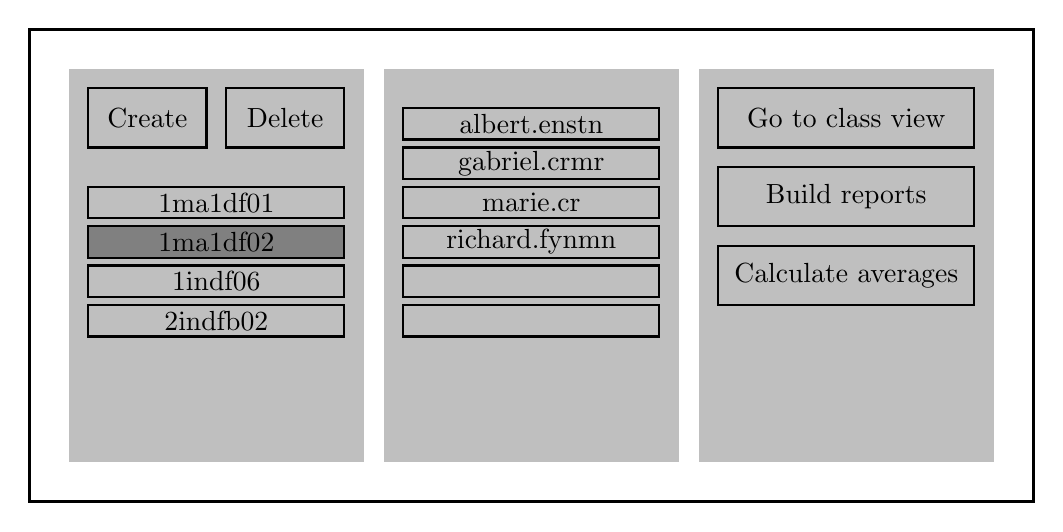
\begin{tikzpicture}

\draw[very thick] (0,0) rectangle (12.75, 6);

\fill[gray!50!white] (0.5, 0.5) rectangle (4.25, 5.5);
\draw[thick] (0.75, 4.5) rectangle (2.25, 5.25) node[pos=0.5] {Create};
\draw[thick] (2.5, 4.5) rectangle (4, 5.25) node[pos=0.5] {Delete};
\draw[thick] (0.75, 3.6) rectangle (4, 4) node[pos=0.5] {1ma1df01};
\draw[fill=gray, thick] (0.75, 3.1) rectangle (4, 3.5) node[pos=0.5] {1ma1df02};
\draw[thick] (0.75, 2.6) rectangle (4, 3) node[pos=0.5] {1indf06};
\draw[thick] (0.75, 2.1) rectangle (4, 2.5) node[pos=0.5] {2indfb02};

\fill[gray!50!white] (4.5, 0.5) rectangle (8.25, 5.5);
\draw[thick] (4.75, 4.6) rectangle (8, 5) node[pos=0.5] {albert.enstn};
\draw[thick] (4.75, 4.1) rectangle (8, 4.5) node[pos=0.5] {gabriel.crmr};
\draw[thick] (4.75, 3.6) rectangle (8, 4) node[pos=0.5] {marie.cr};
\draw[thick] (4.75, 3.1) rectangle (8, 3.5) node[pos=0.5] {richard.fynmn};
\draw[thick] (4.75, 2.6) rectangle (8, 3);
\draw[thick] (4.75, 2.1) rectangle (8, 2.5);

\fill[gray!50!white] (8.5, 0.5) rectangle (12.25, 5.5);
\draw[thick] (8.75, 4.5) rectangle (12, 5.25) node[pos=0.5] {Go to class view};
\draw[thick] (8.75, 3.5) rectangle (12, 4.25) node[pos=0.5] {Build reports};
\draw[thick] (8.75, 2.5) rectangle (12, 3.25) node[pos=0.5] {Calculate averages};


\end{tikzpicture}
\end{center}

Possible events controlled from this view: 
\begin{enumerate}
\item Create a new class.
\item Select the active class.
\item Delete the active class
\item Edit the class list.
\item Pass to the class view of the active class.
\item Build student reports.
\item Calculate average notes.
\end{enumerate}

\subsubsection{Class view}

The class view includes the seating plan, both as a reminder for names and as a visual cue for interactions.

\begin{center}
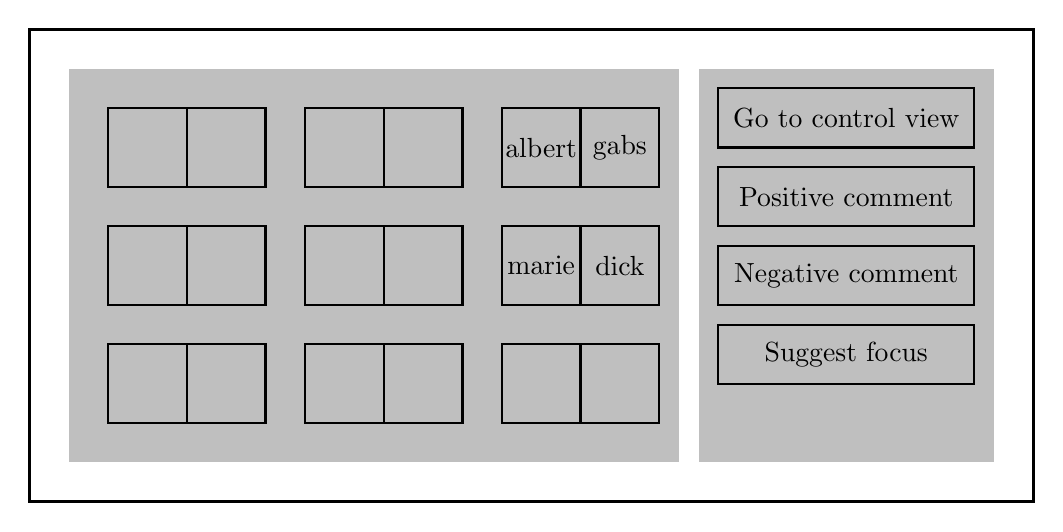
\begin{tikzpicture}

\draw[very thick] (0,0) rectangle (12.75, 6);

\fill[gray!50!white] (0.5, 0.5) rectangle (8.25, 5.5);

\foreach \x in {1,3.5,6} {
\foreach \y in {4,2.5,1} {
\draw[thick] (\x, \y) rectangle (\x+1, \y+1);
\draw[thick] (\x+1, \y) rectangle (\x+2, \y+1);
}
}

\draw[thick] (6, 4) rectangle (7, 5) node[pos=0.5] {albert};
\draw[thick] (7, 4) rectangle (8, 5) node[pos=0.5] {gabs};
\draw[thick] (6, 2.5) rectangle (7, 3.5) node[pos=0.5] {marie};
\draw[thick] (7, 2.5) rectangle (8, 3.5) node[pos=0.5] {dick};

\fill[gray!50!white] (8.5, 0.5) rectangle (12.25, 5.5);
\draw[thick] (8.75, 4.5) rectangle (12, 5.25) node[pos=0.5] {Go to control view};
\draw[thick] (8.75, 3.5) rectangle (12, 4.25) node[pos=0.5] {Positive comment};
\draw[thick] (8.75, 2.5) rectangle (12, 3.25) node[pos=0.5] {Negative comment};
\draw[thick] (8.75, 1.5) rectangle (12, 2.25) node[pos=0.5] {Suggest focus};


\end{tikzpicture}
\end{center}

Possible events: 
\begin{enumerate}
\item Pass back to the control view.
\item Change the seating plan.
\item Select/ deselect a student.
\item Record a positive comment for the selected students.
\item Record a negative comment  for the selected students.
\item Suggest students for next teacher-student focus.
\end{enumerate}

\section{A single executable file}

Ideally, the TAT system would run from a single executable file. The user would launch the TAT application (for example, by double clicking on the icon) and then all interactions would happen through the GUI. 

I tried using two different packages: \textbf{PyInstaller}\footnote{\texttt{https://pyinstaller.org/en/stable/}} and \textbf{cx-Freeze}\footnote{\texttt{https://cx-freeze.readthedocs.io/en/latest/index.html}}. Both packages attempt to build standalone executables from Python scripts by bundling the application and dependencies into a single package. 

Importantly, both scripts are only able to build packages for the hardware and software used when building the package. This means that \textbf{I must build the executable using the school computers,} as the executable I make locally will only run on machines identical to my own. This is a clear disadvantage with the decision to use Python, a scripting language. If I had implemented the TAT system using Java, for example, then I could have assumed the school computers used a compatible virtual machine.

Unfortunately, at this time I have not managed to automate the process of creating a standalone package. PyInstaller has trouble linking to the pygame module, and cx-Freeze dislikes subfolders. Instead I manually create the executable as follows:

\begin{enumerate}
\item Create an empty folder.
\item Copy all the TAT python scripts and the \texttt{requirements.txt} into this folder.
\item Create a virtual Python environment for this directory and add the necessary python modules. This can be done at the command line using

\texttt{pip install -r requirements.txt}

\item Again at the command line in this working directory, run cx-Freeze

\texttt{cxfreeze -c gui.py --target-dir dist}.

\item Copy the \texttt{GUI\_files} directory into the new \texttt{dist} subfolder.
\item From the \texttt{dist} subfolder, zip the following files into a single archive ready for distribution:
\begin{itemize}
\item The application file \texttt{TAT.exe}.
\item The directory of packaged files \texttt{lib}.
\item The directory of TAT options and helper files \texttt{GUI\_files}.
\end{itemize}
\end{enumerate}

\section{Instruction booklet} \label{instructions}

\subsection{Page 1: introduction}

\subsection{Page 2: control view}

\subsection{Page 3: class view}


\section{Missing features} \label{notdone}

Simple executable file

\

instruction booklet

\

exam buttons

\

export seating plan to latex to pdf

\

handling students who leave

\

changing given names after comments already made about them

\

seating plans

\

using the data to make predictions about students. For example: their behaviour in class has changed dramatically (for the better or for the worse); students who might need extra support in order to pass the year; students who should consider accelerated learning programs. There are lots of resources available to the students and to the teachers, and it is difficult for young teachers to suggest

\

Automate the process of creating a standalone package, which is currently manual.

\section{Conclusion}





\begin{thebibliography}{Xyzz12}

\bibitem[Amman16]{Amman16} Ammann, P., \& Offutt, J. (2016). Introduction to software testing. Cambridge University Press.

\bibitem[Anaya18]{Anaya18} Anaya, M. (2018). Clean code in Python. Packt Publishing

\bibitem[Beck03]{Beck03} Beck, K. (2003). Test driven development by example. Addison-Wesley.

\bibitem[Bloom79]{Bloom79} Bloom, B. S. (1976). Human characteristics and school learning. McGraw-Hill.

\bibitem[BCSW10]{BCSW10} Borba, P., Cavalcanti, A., Sampaio, A., \& Woodcook, J. (Eds.). (2010). Testing techniques in software engineering: Second Pernambuco Summer School on Software Engineering, PSSE 2007, Recife, Brazil, December 3-7, 2007, Revised Lectures (Vol. 6153). Springer.

\bibitem[Bryant20]{Bryant20} Bryant, J., Heitz, C., Sanghvi, S., \& Wagle, D. (2020). How artificial intelligence will impact K-12 teachers. Retrieved May, 12, 2020.

\bibitem[BS09]{BS09} Bucheton D. \& Soulé Y. (2009). Les gestes professionnels et le jeu des postures de l’enseignant dans la classe : un multi-agenda de préoccupations enchâssées.

\bibitem[Coad91]{Coad91} Coad, P., Yourdon, E., \& Coad, P. (1991). Object-oriented analysis (Vol. 2). Englewood Cliffs, NJ: Yourdon press.

\bibitem[Hat12]{Hat12} Hattie, J. (2012). Visible learning for teachers: Maximizing impact on learning. Routledge.

\bibitem[Jorg17]{Jorg17} Jorgensen, P. C. (2017). The craft of model-based testing. CRC Press.

\bibitem[Mart08]{Mart08} Martin, R. (2008). Clean Code. Pearson.

\bibitem[Mart17]{Mart17} Martin, R. (2017). Clean Architecture: A Craftsman’s Guide to Software Structure and Design. Pearson

\bibitem[MM78]{MM78} McCorskey, J. C., \& McVetta, R. W. (1978). Classroom seating arrangements: Instructional communication theory versus student preferences. Communication education, 27(2), 99-111.

\bibitem[MSB11]{MSB11} Myers, G. J., Sandler, C., \& Badgett, T. (2011). The art of software testing. John Wiley \& Sons.

\bibitem[Norr98]{Norr98} Norris, J. R. (1998). Markov chains (No. 2). Cambridge university press.

\bibitem[PPDT18]{PPDT18} Le PPDT - Guide pratique RGPD à l'attention des institutions publiques genevoises (2018).


\bibitem[Rob19]{Rob19} Robinson, M. (2019). BOSCARD: A Scoping Tool for Lean Continuous Improvement Projects. In Global Lean for Higher Education (pp. 181-195). Productivity Press.

\bibitem[Swei15]{Swei15} Sweigart, A. (2015). Automate the Boring Stuff with Python.
\end{thebibliography}


\appendix

\section{Original project proposal}

Bucheton and Soulé have described the act of teaching as a multi-agenda game of postures requiring good preparation and excellent micro-decisions \cite{BS09}. In their model, they identify the crucial roles of the teacher in controlling the cadence, the atmosphere, the scaffolding and the relationships during the class, and how each supports the learning objective. And yet many of the teacher's most time-consuming tasks do not take place in the classroom \cite{Bryant20}: good preparation and strong follow-ups (for example auto-reflection, marking and parent-teacher interactions) work to support and complement the pillars identified in the student learning process.

Many of these tasks are ripe for automation. As Sweigart writes, ``many people spend hours clicking and typing to perform repetitive tasks, unaware that the machine they’re using could do their job in seconds if they gave it the right instructions'' \cite{Swei15}.  For my thesis project of the GymInf formation, I intend to build a suite of tools to support a range of teacher tasks including 
\begin{itemize} 
\item organizing seating plans \\
\emph{to aid the atmosphere and relationships} 
\item suggesting teacher-student interactions for upcoming classes \\
\emph{to foster relationships}
\item building individual student reports \\
\emph{to regulate cadence and scaffolding, as well as for follow-ups}
\item creating spreadsheets of marks \\
\emph{for follow-ups}
\end{itemize}
Teachers will interact with the tool using a GUI: it should be easy to use for all teachers, not just those teachers who are computer literate.


I will implement this project using \emph{Test Driven Development.} This is a style of software development that grew out of the `Extreme Programming' philosophy of the 1990s, encouraging quick development cycles and active feedback from clients. The first book written on the subject, \emph{TTD by Example}, by Kent Beck, is still the main resource \cite{Beck03}. Kent emphasises the need to thoroughly test the requirements in order to have confidence when refactoring or making changes, as well as the need to make incremental changes (both for confidence and for time to market). TTD programming follows the following cycle: \\
\indent \textbf{Red.} Write a failing test for a requirement. \\
\indent \textbf{Green.} As quickly as possible, write code to pass the test. \\
\indent \textbf{Refactor.} Clean the code, removing duplication and renaming functions. \\
Coding is driven by testing. In the thesis I will explore testing in more detail.


\section{Useful quotes}
 
\begin{center} 
\emph{``The best climate for learning is one in which there is trust. Students often don’t like to make mistakes because they fear a negative response from peers. Expert teachers create classrooms in which errors are welcome and learning is cool.''} \cite{Hat12}
\end{center}
 
\begin{center} 
\emph{``Since it has been reasonably well established that student affect toward a class is related to student learning, student attitudes toward classroom arrangements are a matter of no small concern when determining a choice of classroom arrangement.''} \cite{MM78}
\end{center}

\begin{verbatim}
https://github.com/zedr/clean-code-python#table-of-contents
\end{verbatim}


\begin{center} 
\emph{``Technology is touted as being able to reduce the time students and teachers spend on menial tasks, time that can be used in other, educationally more meaningful activities. However, there are conflicting views on what is meaningful.''} \cite[p. 11]{Unesco23}
\end{center}

\begin{center} 
\emph{``Successful education systems typically have absorptive capacity, including strong school leaders and confident teachers willing to innovate. Yet often seemingly trivial issues, such as maintenance and repair, are ignored or underestimated.''} \cite[p. 17]{Unesco23}
\end{center}





\end{document}